\documentclass[twocolumn]{article}
\usepackage[top=1.1in, left=0.85in, right=0.85in]{geometry}

% \usepackage{eclbkbox}
\usepackage{amsmath}
\usepackage{amssymb}
% \usepackage{amscd}
% \usepackage{xy}
\usepackage{graphicx}
% \usepackage{fancyhdr}
% \usepackage{color}
% \usepackage[dark,all,bottom,landscape,timestamp]{draftcopy}
% \usepackage{everypage}

% \usepackage{ulem}
% go back to italics for emphasis, though
% \normalem

\begin{document} 

\title{What words ought to exist? \\
       {\normalsize Coining with coinduction}}
\author{Dr.~Tom~Murphy~VII~Ph.D.\thanks{
Copyright \copyright\ 2011 the Regents of the Wikiplia
Foundation. Appears in SIGBOVIK 2011 with the blessing of the
Association for Computational Heresy; {\em IEEEEEE!} press,
Verlag-Verlag volume no.~0x40-2A.
\yen 0.00}
}


\renewcommand\>{$>$}
\newcommand\<{$<$}

\date{3 March 2011}

\maketitle

\begin{abstract}
what do I put here
\end{abstract}

\vspace{1em}
{\noindent \small {\bf Keywords}:
 computational cryptolexicography, n-Markov models, coinduction
}

\section*{Introduction}
During a recent high-stakes game of Scrabble-brand Crossword
Puzzle\footnote{Scrabble is a registered trademark of Hasbro
  Inc./Milton Bradley, and Mattel/JW Spear \& Sons plc.} I had what
could only be described as a killer bingo word (all 7 tiles) that,
after careful study, I determined could not be placed anywhere on the
board. Later in that same game, I had another sequence of letters that
just totally seemed like it should be able to make some long-ass
words, like for example ``oilsoap'' which turns out is not a legal
Scrabble word.\!\footnote{There are actually no 7-letter words that
  can be made from these letters. Don't even bother. Even if playing
  off an existing letter on the board, the best we can do are the
  non-bingos ``topsoil,'' ``topsail,'' or ``poloist'' with an
  available {\it t}.} This naturally made me frustrated and I wanted
to do something about it. Why can't ``oilsoap'' be a word? Or
``loopsia''? Words are introduced into the lexicon all the time. My
first reaction of course was to make an online version of Scrabble
where all words are legal. This is called Scrallbe (where they can
{\it all be} words!\footnote{As of 2011, the official Scrabble slogan
  is ``every word's a winner!'' which is clearly false.}) This is
available at {\tt http://snoot.org/toys/scrallbe}, and is pretty
boring, I gotta be honest (Figure~\ref{fig:scrallbe}).

\begin{figure}
\begin{center}
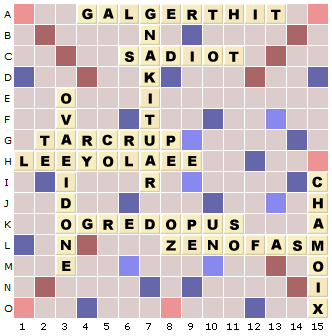
\includegraphics[width=0.75 \linewidth]{scrallbe-screenshot}
\end{center}\vspace{-0.1in}
\caption{In-progress Scrallbe game, 753 points.}
\label{fig:scrallbe}
\end{figure}

The thing is, it's just more fun when some words aren't words. Think
about it: If all words were real, then you could never make a really
devastatingly successful challenge in Scrabble that like, rocked the
whole household and turned a formerly casual family games night into
some kind of crying contest. Spelling bees could still exist, because
while no matter what those kids spelled,\!\footnote{Well, we have to
consider the possibility that the kiddo would use a letter that
doesn't exist. In this particular fantasy, grant me also that every
letter also exists, even $\stackrel{\Diamond}{\smile}$.} it would be
a word, it would not necessarily be the {\it right} word, just like
maybe a homophone. There would be fewer bar fights, but probably not
that many fewer. Moreover, iuhwueg nznie a uaohahweih zmbgba bawuyg!

Clearly we need more words, but not all of them. So this raises the
question: What words {\it ought} to exist? This paper explores several
different approaches for scientifically answering this question,
compares the results, and proposes specific words that should be
added, with their meanings.

Disclaimer possibly indicated for SIGBOVIK: The ``research'' contained
herein is 100\% legitimate.\!\footnote{Source code is available at
{\tt http://tom7misc.svn.
sourceforge.net/viewvc/tom7misc/trunk/wishlist/}} I have attempted to
present it in a tutorial style that assumes little mathematical or
computer science background. I have also left off the last {\it S} for
{\it Savings}.

\section{First idea: Wishlist}

My website ``{\sf snoot.org}'' has a number of games on it, including
a Scrabble clone called Scribble\footnote{{\tt
    http://snoot.org/toys/scribble/}} and Boggle clone called
Muddle.\!\footnote{{\tt http://snoot.org/toys/muddle/}} This website
has been running for almost ten years, comprising over 150,000
Scribble games totaling 3.8 million words placed and 628,000 Muddle
games with over 10 million words found. During each game, players
repeatedly attempt to play words that aren't real. The computer
rebukes them, but hope really springs eternal with these people. It's
like they truly deeply wish to break out of the shackles of the
Official Scrabble Players Dictionary.\!\footnote{For the analyses in
  this paper that depend on a list of legal words, I actually use a
  modified version of SOWPODS, which is the tournament list used in
  Australia and the UK, and significantly more permissive than the US
  Tournament Word List. Though the modified version is non-canonical,
  I stuck with it because it's what's been in use on the site for
  ten years.} So the first approach to determining what
words ought to exist is to analyze the words that people tried to
play, in order to try to extract the essence of word-yearning.

This analysis is quite straightforward. I took the ten years of logs
files and extracted each attempt to play a word in Scribble or Muddle.
These log files are quite large, so the first step is just to get a
count, for each alleged word, and store those in a more convenient
format. There were 3,572,226 total words attempted\footnote{Here a
  word attempted is the major word of the play. This does not include
  incidental words (typically two-letter ones) formed in the
  perpendicular direction.} in Scribble and 13,727,511 in Muddle. The
most frequent ones appear in Figure~\ref{fig:mostfrequent}. Aside from
the one-letter ones, the most frequent words are legitimate words,
since players have a bias towards attempting words that will not be
rebuked by the computer.

Seeing the words that people wish existed is a simple matter of
filtering out the words that already exist, using the Scrabble
dictionary. (I also filtered out one-letter ``words''. It is easy to
see that no one-letter words should exist, again because of
ambiguities created in spelling bees. Not only when literally spelling
``bees'', but according to the official Scripps National Spelling Bee
rules, the speller may optionally pronounce the word to be spelled
before and after spelling it. So if ``s'' were a word, then the
following ridiculous exchange obtains: Judge: ``S. The letter {\it s}.
Etruscan origin.'' Speller: ``S. S. S.'' and the judge cannot tell if
the speller meant to state the word before and after, or thinks the
word is spelled ``sss''.) 22.3\% of the words attempted in Scribble
and 36.8\% in Muddle were not real. The most frequent ones appear in
Figure~\ref{fig:mostfrequentfake}.

\begin{figure}
\begin{center}
\begin{tabular}{|rl@{\qquad}rl|}
\multicolumn{2}{l}{{\bf \large Scribble}} &
\multicolumn{2}{l}{{\bf \large Muddle}} \\
\hline
Count & Word & Count & Word \\
\hline
45,605  &  a        &     20,412  &  late  \\
42,315  &  i        &     19,405  &  rate  \\
32,499  &  d$^*$    &     19,276  &  dear  \\
12,981  &  in       &     19,049  &  tear  \\
12,851  &  oe       &     19,019  &  date  \\
12,528  &  s$^*$    &     18,771  &  lear  \\
12,207  &  re       &     18,423  &  deal  \\
11,159  &  tv       &     18,231  &  real  \\
10,720  &  jo       &     18,138  &  lead  \\
10,386  &  it       &     18,076  &  tale  \\
10,369  &  et       &     17,969  &  lane  \\
9,659   &  qua      &     17,956  &  sear  \\
9,218   &  xi       &     17,570  &  read  \\
9,099   &  go       &     17,193  &  teal  \\
9,052   &  ow       &     17,170  &  lean  \\
8,801   &  qat      &     17,071  &  dare  \\
8,602   &  aa       &     16,923  &  dale  \\
8,278   &  un       &     16,892  &  seal  \\
8,142   &  en       &     16,806  &  sale  \\
8,005   &  or       &     16,465  &  seat  \\
\hline
\end{tabular}
\end{center}
\caption{Most frequently attempted words in Scribble and Muddle. Asterisks
indicate non-words.}
\label{fig:mostfrequent}
\end{figure}

\begin{figure}
\begin{center}
\begin{tabular}{|rl@{\qquad}rl|}
\multicolumn{2}{l}{{\bf \large Scribble}} &
\multicolumn{2}{l}{{\bf \large Muddle}} \\
\hline
Count & Word & Count & Word \\
\hline
11,159 &  tv         &     16,251 &  dane    \\
4,003  &  ok         &     6,156  &  rane    \\
2,862  &  iraq       &     5,603  &  sare    \\
2,725  &  zen        &     5,576  &  nate    \\
2,448  &  cho        &     4,863  &  mear    \\
1,538  &  viz        &     4,750  &  cale    \\
1,418  &  sdasda     &     4,616  &  nees    \\
1,396  &  von        &     4,568  &  nale    \\
1,136  &  etc        &     4,507  &  fale    \\
878    &  int        &     4,347  &  deat    \\
829    &  june       &     4,263  &  tean    \\
745    &  lp         &     4,251  &  nile    \\
719    &  zion       &     4,160  &  mens    \\
665    &  cia        &     4,087  &  deel    \\
661    &  jim        &     3,851  &  deam    \\
651    &  iraqi      &     3,828  &  dana    \\
648    &  ques       &     3,781  &  beed    \\
542    &  que        &     3,769  &  lans    \\
502    &  tim        &     3,725  &  tade    \\
\hline
\end{tabular}
\end{center}
\caption{Most frequently attempted non-words in Scrabble and Muddle.}
\label{fig:mostfrequentfake}
\end{figure}

There's a clear difference between these two lists. The Scribble list
is dominated by words involving difficult-to-play letters like {\it v}
(there are no legal two-letter {\it v}-words). Most of the words would
probably be acknowledged as real, just not legal in Scribble. The ones
that don't already have meanings, like ``cho'' and ``int'' and ``que''
seem to be pretty good candidates to exist. The Muddle list is all
four-letter words (the minimum allowed length) using common letters.
Other than the ones that are already words, like ``dane'' and ``nile''
and ``mens'' (as in ``mens section'' or ``the powerfuel weapon kills
hard so many mens''), these are all good candidates for words to
exist. Probably if you were playing someone really intense in
Scrabble, and he or she played one of these, and was super deadpan
about it and maybe had caused some crying contests before, and a known
sesquipedalianist, you would let these fly because they look like real
words to me. A point in their favor is that they would be quite
low-scoring words in Scrabble; not a {\it z} or {\it q} to be found.
Even in the Scribble list there's no ``qzkwv'' junk. The effect is
probably due to a few factors: Players are less likely to attempt
obvious non-words, common letters appear more often on the rack and on
the board and so the opportunity to play words like in
Figure~\ref{fig:mostfrequentfake} presents itself more frequently, and
in Muddle, there is no advantage to using unusual letters, except the
joy of being a weirdo. Nonetheless, these lists are surely biased by
the specifics of Scribble and Muddle, and the question at hand is not
just what words ought to exist for the purpose of internet word games,
but for general purposes.

\begin{figure}
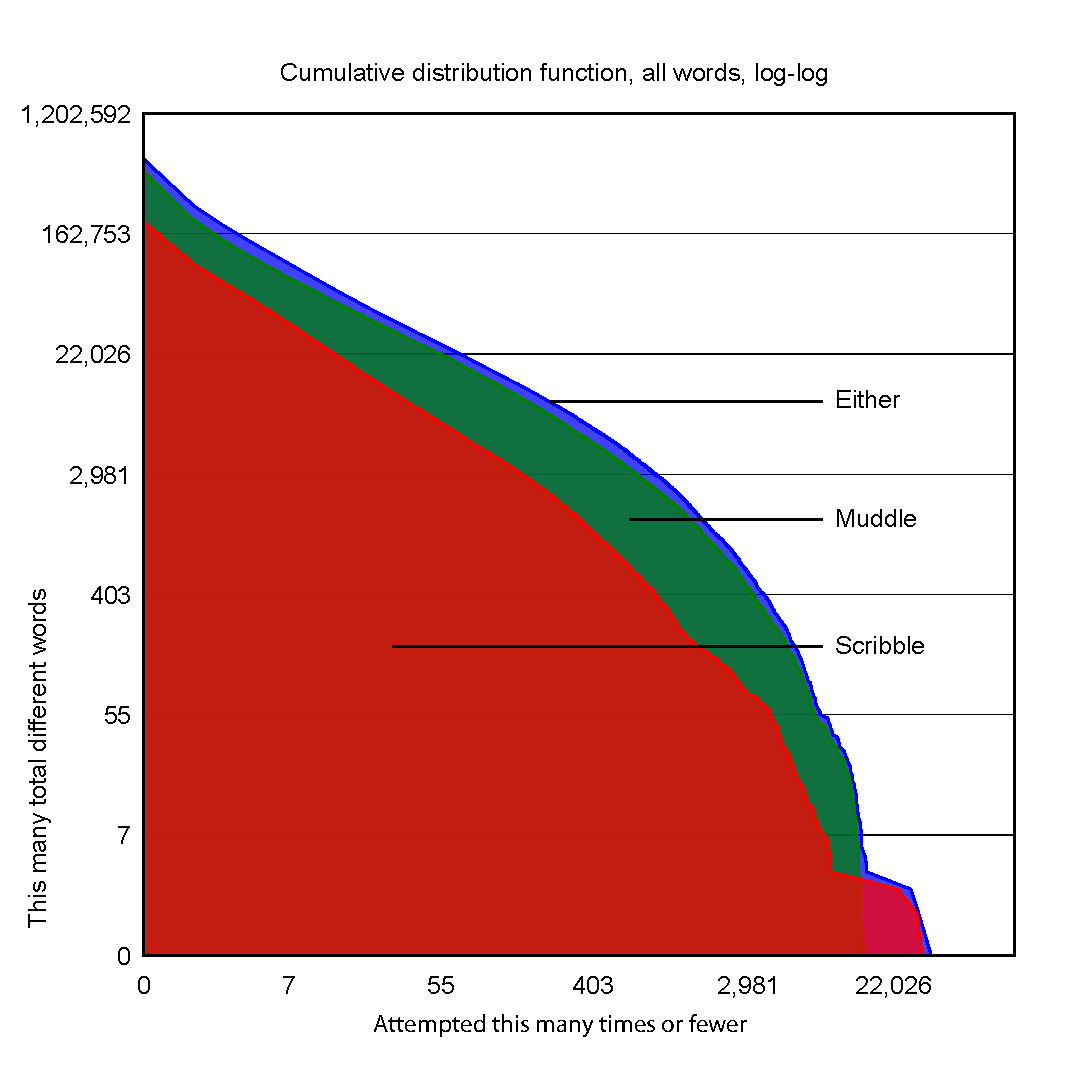
\includegraphics[width=\linewidth]{wishlist-cdf}
\caption{Distribution of word frequency. Approximately 25,000
  different words (y axis) were issued 55 times or fewer (x axis).}
\label{fig:gamedistribution}
\end{figure}

Another downside is that this method completely ignores the many words
that are attempted only once or a small number of times. Players are
very creative; of the 564,610 unique words attempted, 501,939 of them
aren't real! The vast majority of words are attempted only a handful
of times (Figure~\ref{fig:gamedistribution}). Though those words
individually are not good candidates to exist, like tiny stars wished
upon in the night sky,\!\footnote{Astronomers now agree that stars do
  exist, by the way.} in aggregate they form a significant planetarium
that may tell us what {\it kind} of words people wish existed. For
example, if we saw that the words ``sweeeeeeet'',
``sweeeeeeeeeeeeet'', ``sweeeet'' and ``sweeeeeeeeeeeeeet'' occurred a
few times each, we could infer that people wished that words like
``sweet'' with strictly more than two {\it e}s were real words. They
might even be indifferent to the absolute number of {\it e}s, as long
as there existed some legal variation with more than two {\it e}s.
(This appears to be borne out by data. According to Google's
estimates, the words ``swe$^n$t'' for various medium-sized $n$
(10--20) appear on the Internet with similar frequency. The only
exception is ``sweeeeeeeeeeeeeeeeeeet'', with 19 {\it e}s, which
unexpectedly appears three times as often as 18 or 20 {\it e}s does;
see Figure~\ref{fig:sweet}.) In order to lance these two boils, in the
next section I explore statistical methods for generalizing from lots
of individual examples.

% XXX should really try to get this in the right column, since it
% overflows the margins
\begin{figure}
\begin{tabular}{r|r|l}
17,900,000 & 0 & swt \\
1,060,000 & 1 & swet \\
580,000,000 & 2 & sweet \\
1,310,000 & 3 & sweeet \\
806,000 & 4 & sweeeet \\
509,000 & 5 & sweeeeet \\
283,000$^1$ & 6 & sweeeeeet \\  % spell correction for five
170,000 & 7 & sweeeeeeet \\
115,000 & 8 & sweeeeeeeet \\
75,200 & 9 &  sweeeeeeeeet \\
94,300$^2$ & 10 & sweeeeeeeeeet \\ % spell correction for nine?
51,700 & 11 & sweeeeeeeeeeet \\
37,900 & 12 & sweeeeeeeeeeeet \\
32,000 & 13 & sweeeeeeeeeeeeet \\
25,300 & 14 & sweeeeeeeeeeeeeet \\
24,300 & 15 & sweeeeeeeeeeeeeeet \\
41,000$^3$ & 16 & sweeeeeeeeeeeeeeeet \\ % spell correction for 14
55,000 & 17 & sweeeeeeeeeeeeeeeeet \\
45,000 & 18 & sweeeeeeeeeeeeeeeeeet \\
133,000$^4$ & 19 & sweeeeeeeeeeeeeeeeeeet \\ % for 15
34,800 & 20 &  sweeeeeeeeeeeeeeeeeeeet \\
%
16,100$^5$ & 25 & sweeeeeeeeeeeeeeeeeeeeeeeeet \\ % for weeeeeeeeeeeeeeeeeeeeeeeee t
10,100 & 30 & sweeeeeeeeeeeeeeeeeeeeeeeeee\ldots t \\
2,800 & 40 &  sweeeeeeeeeeeeeeeeeeeeeeeeee\ldots t \\
923 & 50 &    sweeeeeeeeeeeeeeeeeeeeeeeeee\ldots t \\
118 & 75 &    sweeeeeeeeeeeeeeeeeeeeeeeeee\ldots t \\
38 & 100 &    sweeeeeeeeeeeeeeeeeeeeeeeeee\ldots t  \\
?$^6$ & 200 & sweeeeeeeeeeeeeeeeeeeeeeeeee\ldots t     \\ % word is too long for Google
\end{tabular}
\caption{Frequency of ``swe$^n$t'' on the internet for various $n$, estimated
by Google. Notes: {\bf (1)} Spell correction offered for ``sweeeeet''. {\bf (2, 3, 4)} Spell corrections
offered to e$^{9}$, e$^{14}$ and e$^{15}$ respectively. {\bf (5)} Spell correction offered for ``weeeeeeeeeeeeeeeeeeeeeeeee t'' (?) {\bf (6)} With two hundred {\it e}s, the word is too long for Google, which asks me to ``try using a shorter word.'' Thanks Google, but I already did try the shorter ones.}
\label{fig:sweet}
\end{figure}

\section{Statistical Models}

The reason that people are more likely to play words like ``rane'' is
that the letters are common---they appear more often in words, and
more often in the Scrabble bag. But it's not simply a matter of the
frequency of letters; if it were, we would expect to see words like
``eee'' dominating the list, since {\it e} is the most common letter
in English.\!\footnote{Tied for first place with {\it n}, {\it g},
{\it l}, {\it i}, {\it s}, and {\it h}.} People do not play such words
often because they do not {\it seem} like real words. ``oilsoap''
seems more like a word than ``ioaopsl'' to most non-crazy people,
even though they contain the same letters. This is because we have
expectations on what letters are likely to appear next to one
another in words. This section is about modeling expectations on
what letters appear together, and then using that model to generate
the most likely words that don't yet exist.

{\bf Markov chains.}\,
This guy called Andrei Markov had an idea which is pretty obvious in
retrospect, but he had it like a hundred years ago before any of us
were born (probably; if not: you are old), which he didn't call Markov
chains but now they're called Markov chains because I guess in the
hopes that contemporary mathematicians will get stuff named after
their dead selves if they keep the tradition of naming stuff after
dead people alive. The idea is easiest to understand in the context
of the current problem. Suppose we know that the words ``hello'',
``helpful'' and ``felafel'' are the only real words. The following
is a frequency table of how often each letter occurs.

\begin{center}
\begin{tabular}{|r|r|r|r|r|r|r|r|} % {helopfua}
\hline
h   & e   & l   & o   & p   & f   & u   & a    \\
\hline
2   & 4   & 6   & 1   & 1   & 3   & 1   & 1    \\
\hline
\end{tabular}
\end{center}

This tells us that {\it l} is by far the most common letter, so the
most likely word is probably ``l'' or ``llllllll'' or something. A
Markov chain is like a frequency table, but instead of counting
individual letters, we count how often one letter comes {\it after}
another. Here is the Markov chain for those words.

% of the current problem. Suppose we know that the words ``hello'',
% ``helpful'' and ``felafel'' are the only real words. The following

\begin{center}
\begin{tabular}{|c|r|r|r|r|r|r|r|r|} % {helopfua}
\hline
\,  &  {\bf h}   & {\bf e}   & {\bf l}   & {\bf o}   & {\bf p}   & {\bf f}   & {\bf u}   & {\bf a} \\
\hline  %    h     e     l     o     p     f     u     a
{\bf h}   &  0   & 0   & 0   & 0   & 0   & 0   & 0   & 0    \\
\hline
{\bf e}   &  2   & 0   & 0   & 0   & 0   & 2   & 0   & 0    \\
\hline
{\bf l}   &  0   & 4   & 1   & 0   & 0   & 0   & 1   & 0    \\
\hline
{\bf o}   &  0   & 0   & 1   & 0   & 0   & 0   & 0   & 0    \\
\hline
{\bf p}   &  0   & 0   & 1   & 0   & 0   & 0   & 0   & 0    \\
\hline
{\bf f}   &  0   & 0   & 0   & 0   & 1   & 0   & 0   & 1    \\
\hline
{\bf u}   &  0   & 0   & 0   & 0   & 0   & 1   & 0   & 0    \\
\hline
{\bf a}   &  0   & 0   & 1   & 0   & 0   & 0   & 0   & 0    \\
\hline
\end{tabular}
\end{center}

The letters across the top are the ``previous letter'' and the ones
across the left are the ``next letter'' and the box contains the
corresponding count. For example, the pair ``el'' appears four times.
(Pairs of letters are called ``bigrams'' by nerds, some nerd-poseurs,
and Markov who I can't tell if he was a nerd by his picture, because
he does have a pretty austere beard, but also did a lot of math.) One
of the useful things about a Markov chain is that it lets us predict
the next letter that we might see. For example, if we see ``half'',
then the column labeled {\bf f} above tells us that the next letter is
twice as often an {\it e} than a {\it u}, and that no other letters
ever occurred. Typically we think of these as being probabilities
inferred from our observations, so we say there's a 2/3 chance of {\it
e} following {\it f} and a 1/3 chance of {\it u}. Now the word ``llllll''
isn't so likely any more, because there's only a 1/4 chance of the
next letter being {\it l} once we see {\it l}.

Words are not just their interiors; it's also important what letters
tend to start and end words. We can do this by imagining that each
word starts and ends with some fake letters, and include those in the
Markov chain. Let's use {\bf \<} for the start symbol and {\bf \>} for
the end. So we pretend we observed ``\<hello\>'', ``\<helpful\>'', and
``\<felafel\>''. Speaking of which, could you imagine if there were such
a thing as a helpful felafel? Would you eat it? Because then it
probably can't help you any more, except to get fat.

\begin{center}
\begin{tabular}{|c|r|r|r|r|r|r|r|r|r|} % {helopfua}
\hline
\,  &  {\bf \<}    & {\bf h}   & {\bf e}   & {\bf l}   & {\bf o}   & {\bf p}   & {\bf f}   & {\bf u}   & {\bf a}    \\
\hline  %  \<     h     e     l     o     p     f     u     a
{\bf h} &  2  &  0   & 0   & 0   & 0   & 0   & 0   & 0   & 0    \\
\hline    
{\bf e} &  0  &  2   & 0   & 0   & 0   & 0   & 2   & 0   & 0    \\
\hline    
{\bf l} &  0  &  0   & 4   & 1   & 0   & 0   & 0   & 1   & 0    \\
\hline    
{\bf o} &  0  &  0   & 0   & 1   & 0   & 0   & 0   & 0   & 0    \\
\hline    
{\bf p} &  0  &  0   & 0   & 1   & 0   & 0   & 0   & 0   & 0    \\
\hline    
{\bf f} &  1  &  0   & 0   & 0   & 0   & 1   & 0   & 0   & 1    \\
\hline    
{\bf u} &  0  &  0   & 0   & 0   & 0   & 0   & 1   & 0   & 0    \\
\hline    
{\bf a} &  0  &  0   & 0   & 1   & 0   & 0   & 0   & 0   & 0    \\
\hline    
{\bf \>} &  0  &  0   & 0   & 2   & 1   & 0   & 0   & 0   & 0    \\
\hline
\end{tabular}
\end{center}

We just added these like other letters, but since the beginning symbol
{\bf \<} never occurs after other letters, we don't need a row for it
(it would be all zeroes), and similarly since no letters ever follow
{\bf \>} we don't need a column for it. Now the word ``lllll'' is
impossible because no words start with {\it l}.

It basically makes sense to consider the probability of a whole word
to be the chance of simultaneously seeing each pair of letters in it,
which is just the product of all the probabilities. So the word
``hel'' is $2/3$ (for {\bf \<h}) $\times$ 2/2 (for {\bf he}) $\times$
4/4 (for {\bf el}) $\times$ 2/6 (for {\bf l\>}), which is $0.222$.
These are the most likely words overall (I discuss how to generate
such lists in Section~\ref{sec:coin}):

\begin{center}
\begin{tabular}{rl@{\quad\quad}rl}
22.2\%  &  hel      &      2.5\%  &  helpfel  \\
11.1\%  &  helo     &      2.5\%  &  helafel  \\
 7.4\%  &  fel      &      1.9\%  &  fulo     \\
 3.7\%  &  hell     &      1.9\%  &  hello    \\
 3.7\%  &  felo     &      1.2\%  &  fell     \\
 3.7\%  &  ful      &      1.2\%  &  helafelo \\
\end{tabular}
\end{center}

This is pretty good. These words resemble the ones we observed to build
the Markov chain, but are novel. I think helafelo is a pretty rad word,
right?

\begin{figure}
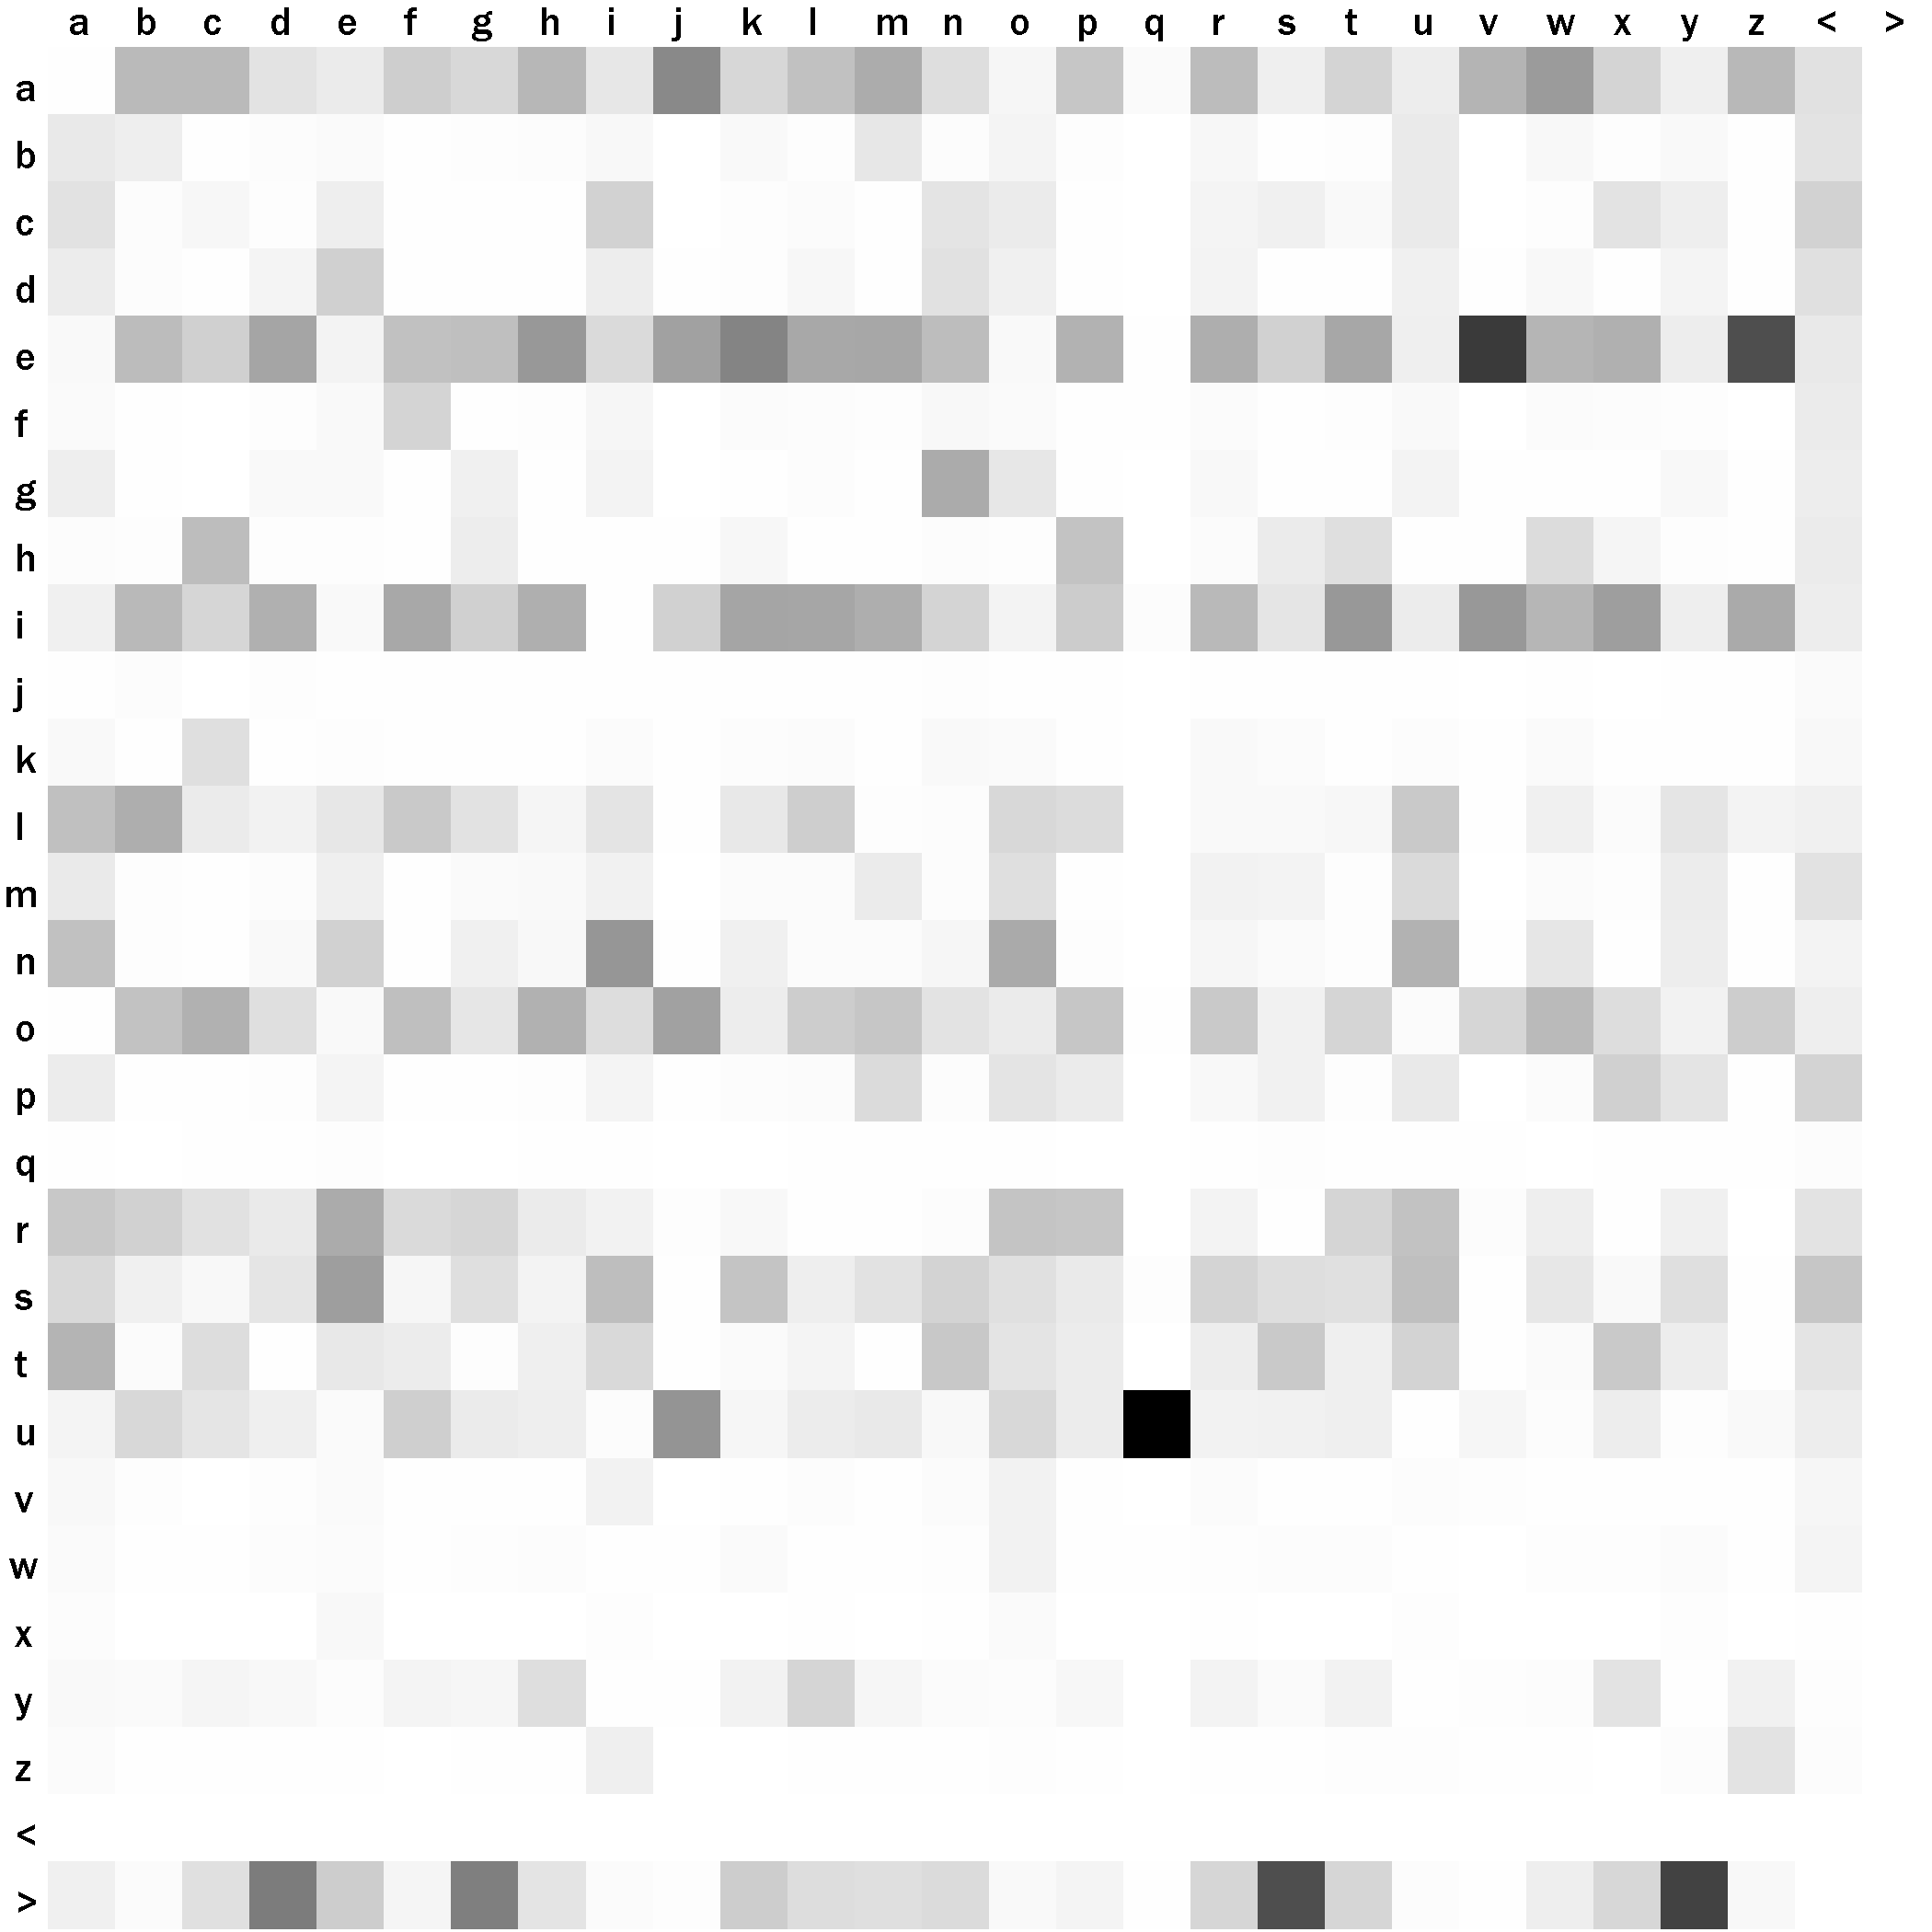
\includegraphics[width=\linewidth]{coin1}
\caption{Markov chain for the SOWPODS word list, where darker squares
indicate higher probability. The darkest is the transition from {\it q}
to {\it u} ($98\%$), which is not surprising.}
\label{fig:sowpodsbigrams}
\end{figure}

The next step is to build a Markov chain for a list of real words and
see what results. I built one for the SOWPODS word list, which results
in the table in Figure~\ref{fig:sowpodsbigrams}. These
are the most likely words, with real words filtered out:

% XXX improve layout
\begin{center}
\begin{tabular}{rl@{\quad\quad}rl}
0.049901545  & s     &   0.001768358  & y   \\
0.017526947  & d     &   0.001761301  & p   \\
0.009521421  & g     &   0.001653041  & a   \\
0.005506083  & c     &   0.001652864  & n   \\
0.004376836  & r     &   0.001563810  & ps  \\
0.004218223  & t     &   0.001383503  & ms  \\
0.004088377  & e     &   0.001371545  & ts  \\
0.003560976  & m     &   0.001327023  & ds  \\
0.003248559  & ss    &   0.001188715  & hy  \\
0.002001529  & rs    &   0.001166457  & k   \\
0.001958674  & h     &   0.001160619  & ng  \\
0.001873761  & l     &   0.001142785  & ly  \\
\end{tabular}
\end{center}


Ugh, poop city! Actually, it turns out that when you see enough words,
you see enough pairs that all sorts of junk looks likely. For example,
``ng'' is easily explained by many words starting with {\it n}, {\it
g} often following {\it n}, and many words ending with {\it g}. Even
though each pair makes sense, the whole thing doesn't look like a word,
because we expect to at least see a vowel at some point, for one thing.

There is a standard solution to this problem, which is to generalize
the Markov chain to keep more than one letter of history. So instead
of just tallying how often {\it g} follows {\it n}, we count how often
{\it g} follows {\it in} (and any other pair of letters).\!\footnote{
  The details are straightforward, except possibly that we now imagine
  each word to start with two (or in general, $n$) copies of the start
  symbol, so that we see ``\<\<helpful\>''. The column corresponding
  to the history {\bf \<\<} tells us the frequency of letters that
  start words, and for example the column {\bf \<h} tells us the
  frequency of letters that follow {\it h} when it appears at the
  start of a word. We do not need to repeat the ending character \>
  because once we see it, we never do anything but end the word.} This
makes the table pretty large, so you'll just have to look at
Figure~\ref{fig:sowpodsbigrams} again and imagine it being 28 times
wider. But the good news is that it invents much better words:

\begin{verbatim}
Markov chain with n=2.
100 top paths:
0.007092576 ing
0.002483309 ses
0.001694275 des
0.001548279 nes
0.001403047 sts
0.001314279 se
0.001287353 ings
0.001262904 ded
0.001170356 cal
0.001101124 le
0.001078157 der
0.001070769 ove
0.001016514 gly
0.000882527 hy
0.000853499 ung
0.000838535 cy
0.000816757 pres
0.000802384 pers
0.000787731 ps
0.000771953 ders
0.000746855 ly
0.000732157 ines
0.000709460 ve
0.000650273 sm
0.000650062 ty
0.000642246 pred
0.000627432 ble
0.000622587 hed
0.000603012 ter
0.000587263 gy
0.000564629 sms
0.000549088 py
0.000545497 ans
0.000541832 ber
0.000531745 ce
0.000489139 ang
0.000487316 unt
0.000482908 snes
\end{verbatim}

\begin{verbatim}
Markov chain with n=3.
100 top paths:
0.001093377 des
0.000789743 pers
0.000767821 cal
0.000622381 pres
0.000452415 nons
0.000449855 ress
0.000426892 ing
0.000404454 pred
0.000387570 ent
0.000366753 dist
0.000357115 ble
0.000353576 ches
0.000348642 gly
0.000345564 inted
0.000340691 dists
0.000339750 lity
0.000336468 und
0.000331914 dises
0.000331389 int
0.000320104 ints
0.000291846 ching
0.000284350 tely
0.000284228 dise
0.000279669 ster
0.000279431 ves
0.000276676 stic
0.000272655 tric
0.000263922 cally
0.000261415 ter
0.000260898 ents
0.000258270 rous
0.000253990 dising
0.000245834 phy
0.000244272 dised
0.000240505 hous
0.000239726 resses
0.000237100 sters
0.000236753 ove
0.000230976 dism
0.000227701 ched
0.000225104 fing
0.000222993 ence
0.000221624 ters
0.000219511 disms
0.000219246 unders
\end{verbatim}

\begin{verbatim}
Markov chain with n=4.
100 top paths:
0.000454575 unders
0.000341807 dising
0.000293774 pers
0.000285248 cally
0.000232842 inted
0.000204856 heter
0.000198642 tric
0.000188363 ster
0.000185238 hier
0.000183216 unded
0.000174876 heters
0.000169220 sters
0.000153800 stic
0.000142753 pering
0.000132595 dises
0.000131040 ching
0.000129387 shing
0.000125442 dest
0.000115038 teless
0.000113312 resis
0.000112909 dist
0.000112793 dists
0.000112397 mising
0.000109589 sation
0.000109555 fing
0.000108931 dised
0.000107632 ches
0.000102999 cated
0.000101327 dise
0.000097730 sations
0.000096676 inding
0.000095270 nons
0.000093852 lary
0.000093357 ency
0.000091199 ther
0.000090608 ories
0.000090405 alled
0.000088604 apped
0.000088235 hous
0.000087780 trous
0.000082438 undered
0.000081713 noning
0.000079613 dism
0.000079071 thers
0.000078380 ented
0.000076765 irred
0.000076363 disms
0.000074970 geness
0.000074910 veness
0.000071079 vities
0.000070308 mised
0.000068585 ques
0.000068096 unding
0.000067618 sher
0.000067429 peries
\end{verbatim}

\begin{verbatim}
n=5
GetTempFileName failed with error 5
\end{verbatim}

Wikipedia favorites: smally (.000287),
websity (.000156),
stude (.000156),
chool (.000124),
fontry (.000120),
undex (.000102),
octory (.0000990),
coibot (.0000960),
footnot (.0000837),
reporth (.0000518),
delection (.0000484),
grounty (.0000459),
betweek (.0000437),
fination (.0000431),
manuary (.0000388),
whicle (.0000360),
stategory (.0000262),

% laplace smoothing?
% TODO: the empty string?

TODO: most likely words in italian, too.

% word list from Italian Scrabble, which I bet is called
% {Scrabbizzimo!}

\subsection{Coining words with coinduction} \label{sec:coin}

In the earlier sections I blithely produced tables of the most
probable words according to an $n$-Markov chain. It is not obvious how
to do this (or that it is even possible), so I explain the algorithm
in this section. It's safely skippable, I mean if you don't want to
know about a pretty cool algorithm that's not that complicated and
might even be new, plus {\em dual math}.

Computing the probability of an individual word is easy. We prefix it
with $n$ copies of the start symbol \<, suffix it with a single \>,
and then look up the probability of each symbol given its $n$
preceding symbols in the table, and multiply those all together. We
can compute the probability of any word this way. The problem with
sorting all of the possible words by their probabilities is that there
are an infinite number of them. We can't just look at short words
first, either, because for example the word ``thethethe'' is many
times more likely ($p = 6.08\times 10^{-11}$) than the shorter
``qatzs'' ($9.07\times 10^{-12}$).

The solution is to use coinduction. Most people remember induction
from school, maybe, which is the one where you have some base case
like ``0 is even'', and then you prove that all numbers are either
even or odd by assuming ``$n$ is even or odd'' and proving ``$n + 1$
is even or odd''. 

most people remember induction, perhaps 
coinduction: never gonna give you up. once you pop you can't stop.


\section{Survey}

On occasion I have been accused of ``overthinking'' problems, whatever
that means. So to compare, I next hazarded a tried and true technique
from grade school, the survey.

Rob: etsy, nuuog
Chris: tapping on the bisphenol-A, nurm
David: wafflucinations
Lea: hnfff sound
Reed: pansepticon
Jessica: gruntle (like not disgruntled)

In order to not reprint everyone's bullshit---but not introduce bias by selectively removing data---I discarded random subsets of the data until it did not contain bullshit any more.

% TODO: backformation, stripping dis- and anti- and un- from words
% then checking to see if they're still words?

% TODO: portmanteautally

% ``Scrallbe'' is kind of like god mode for scrabble.

\section{Recommendations}

sweeeeeeeeeeeeeeeeeeet with 19 {\it e}s, which means ``Really sweet.''

``rane'' sounds too much like ``rain'', but ``sare'' has a unique pronunciation and many people seem to think it's already a word. ``cho'' is similarly easy to pronounce and spell. I propose that it be defined as ``A kind of cheese,'' so that we can really nail the new triple entendre on the classic joke.

% \begin{Verbatim}
facebook wall posts, 4-grams
100 top paths:
0.002525504 pittsburgh
0.002093510 steelers
0.002093510 sfo
0.001953943 it's
0.001256106 bdl
0.001116539 sigbovik
0.001099196 facebook
0.000976971 mic
0.000976971 s
0.000976971 can't
0.000837404 i'm
0.000837404 icfp
0.000837404 app
0.000697837 x
0.000697837 drunj
0.000697837 g
0.000616021 ther
0.000558269 doesn't
0.000558269 's
0.000558269 sr
0.000558269 pm
0.000558269 fyi
0.000558269 wtf
0.000558269 k
0.000558269 don't
0.000558269 today's
0.000558269 m
0.000558269 what's
0.000456766 iphone
0.000429438 inted
0.000418702 oh
0.000418702 phl
0.000418702 gonna
0.000418702 pre
0.000418702 zrh
0.000418702 th
0.000418702 h
0.000418702 b
0.000418702 n
0.000418702 ok
0.000418702 d
0.000418702 that's
0.000418702 rex
0.000418702 fanzibar
0.000418702 st
0.000418702 kinda
0.000418702 didn't
0.000355262 cally
0.000334962 brillobox
0.000314027 superburrito
0.000305304 weath
0.000279135 techno
0.000279135 vii


trigrams, including comments:
100 top paths:
0.003013897 it's
0.001856422 ther
0.001704432 i'm
0.001503910 sfo
0.001102867 -
0.001102867 oh
0.001050350 don't
0.001002607 haha
0.001002607 s
0.000902346 bdl
0.000808769 mic
0.000808769 that's
0.000776981 pittsburgh
0.000705812 thes
0.000701825 ok
0.000645063 can't
0.000601564 icfp
0.000601564 k
0.000583335 didn't
0.000507201 runj
0.000501303 g
0.000501303 omg
0.000501303 x
0.000485262 ins
0.000453126 sout
0.000450580 ands
0.000449950 coff
0.000425932 reat
0.000425133 ning
0.000416189 pittle
0.000412468 getty
0.000407151 ster
0.000401043 sr
0.000401043 pm
0.000401043 m
0.000401043 wtf
0.000401043 aw
0.000401043 d
0.000401043 fyi
0.000401043 ple
0.000401043 's
0.000400791 phon
0.000386315 weat
0.000384116 befor
0.000375978 els
0.000374307 als
0.000357782 nothe
0.000354769 app
0.000354769 appy
0.000354422 they're
0.000353750 wate
0.000345727 there's
0.000340508 res
0.000339344 mes
0.000334202 ove
0.000326473 wher
0.000324373 lity
0.000319011 hotos
0.000316613 dea
0.000315777 sigbovik
0.000315105 ver
0.000314965 thand
0.000310607 outh
0.000300782 n


facebook, n = 2
100 top paths:
0.010628671 ing
0.007144197 th
0.005025442 st
0.004291375 re
0.002932937 ne
0.002662094 se
0.002546194 whe
0.002108786 ther
0.001923496 al
0.001669458 con
0.001652820 wor
0.001498222 ch
0.001495485 wis
0.001379778 i'm
0.001336166 jus
0.001302469 sh
0.001280888 yout
0.001244352 fo
0.001225250 le
0.001224422 pre
0.001221357 ar
0.001201881 com
0.001200574 ge
0.001165417 thes
0.001116295 som
0.001108305 fing
0.001104851 ang
0.001102867 -
0.001102706 it's
0.001039704 ist
0.001036886 hing
0.001007930 ou
0.001002607 s
0.000967282 de
0.000932965 en
0.000926568 tor
0.000827260 wat
0.000827151 oh
0.000814235 cor
0.000812961 ned
0.000783696 lis
0.000762020 ple
0.000760162 whis
0.000759898 sed
0.000755396 res
0.000728412 mor
0.000728049 ong
0.000727818 don
0.000720098 cand
0.000710277 ning
0.000708380 ithe
0.000693547 ame
0.000659248 ty
0.000656211 dow
0.000635771 ha
0.000633225 ext
0.000601564 k
% \end{Verbatim}

% Paper ends with a bigram summary of itself.

% Paper ends with a word that is obviously missing a final 's'.


\end{document}
